%!TEX root = ../construction.tex
% -*- root: ../construction.tex -*-

\begin{comment}
Today's industries are using the power of ubiquitous technologies and human computer interaction (HCI) technology to make work as seamless as possible. Especially in the field of modern architecture, architects are using new computing technology to enhance creativity and aid in communication between various stakeholders. Still, construction engineers on-site may not be familiar with new technology and instead use old-fashion tools to understand the architect's drawings. As a result, management and communication of the architect's design plan may not be followed according to his or her overall specifications which can cause increase in budget costs, confusion in safety factors, and poor building design.
A number of studies using enhanced IT technologies have been developed to help manage and communicate the task of acquiring real-time information that may not otherwise be available on hand. These technologies must be designed to be portable or wearable so they can be used on-site\cite{song_penlight:_2009, yeh_-site_2012}, and must offer intuitive use of 3D data so they can easily map 3D spaces in the real world \cite{chi_research_2013, kim_interactive_2012, yeh_-site_2012}. They also need interfaces for input of modifications in order to reflect adjusted or updated information occurring on-site in the overall model in real-time\cite{song_penlight:_2009}, and integrated BIM technology is important to combine entered information and keep the overall model's information consistent. 
In this paper, we applied \textit{interactive 3D Smart Sapce}\cite{grossman__2010} and \textit{Mobile Computing} to solve the portability problem and providing a feasible interface for on-site construction work. To make our system portable, we used a small depth camera and portable projector to recognize the geometry of the world and to project additional information. Using an 'L'-shape wall presents at work sites, our system projects content onto a vertical wall and horizontal surface allowing 2D interaction to take place on the horizontal surface and 3D interaction on the wall. This natural user interface (NUI) makes for an intuitive aid in construction work providing additional 3D information to interact with. 


In addition, we incorporate the use of an Anato Pen to allow the user to make modifications in real-time while on the job site. We conducted an informal study with participants who are involved in the construction process to evaluate our system. The remainder of this paper examines the feedback from the participants, implementation and experiment results of the drawing functions. Furthermore, construction information can be seen on the work site using a mobile phone. Using this system, seamless information sharing and integration are offered between mobile phones through a shared workspace, Interactive 3D Smart Space and personal workspace. Through this, construction information can be used seamlessly on the construction site as well while the construction model information is updated in real-time with this system designed to enable convenient on-the-job cooperation. The system in this paper is designed for application on construction sites, and after use, informal user studies were conducted on construction managers to verify the usefulness of this system through comparative research. Additionally, experiment feedback and difficulties in realizing the experiment were considered to infer a conclusion.
\end{comment}

Today's industries use ubiquitous computing and human computer interaction technologies to make work as seamless as possible. Especially in modern architecture, architects are using new computing technology to enhance creativity and aid in communication between various stakeholders. Nevertheless, construction engineers on site might not be familiar with new technology, using old-fashioned tools to understand an architect's drawings. As a result, management and communication of an architect's design plan might not be conducted according to his or her overall specifications, potentially causing increased budget costs, confusion in safety factors, and poor building design. A number of studies using enhanced information technologies have been developed to help manage and communicate the acquisition of real-time information that might not be available otherwise. These technologies must be designed to be portable or wearable to enable them to be used on site \cite{song_penlight:_2009, yeh_-site_2012} and must offer intuitive use of 3D data to enable easy mapping of 3D spaces in the real world \cite{chi_research_2013, yeh_-site_2012}. They also need interfaces for input of modifications to reflect information adjusted or updated on site in the overall model in real-time \cite{song_penlight:_2009}, and integrated building information modeling (BIM) technology is important to combine entered information and keep the overall model's information consistent. 

\begin{figure}[b!]
\centering
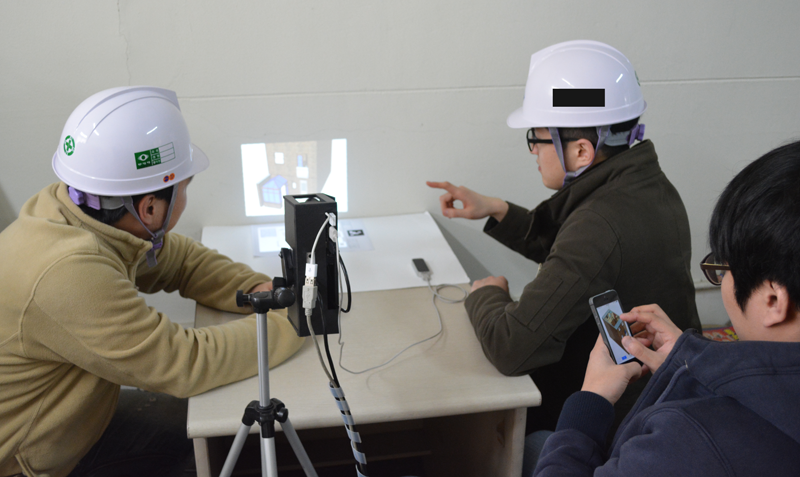
\includegraphics[width=1.0\columnwidth, height=5cm]{1-Introduction/proposed_system}
\caption{Prototype of Port3DAr}
\label{fig:prototype}
\end{figure}
\modified{In this paper, we combine interactive 3D smart spaces \cite{grossman__2010} and mobile computing to solve the portability problem and provide a feasible interface for on-site construction work. To make our system portable, we used a portable depth camera and projector to recognize the geometry of the world and to project additional information. Using an L-shaped wall present at work sites, our system projects content onto a vertical wall and horizontal surface, allowing 2D interaction to take place on the horizontal surface and 3D interaction on the wall. This natural user interface (NUI) provides an intuitive aid in construction work and additional 3D information to interact with. In addition, we incorporate the use of an Anoto Pen to allow the user to make modifications in real-time while on the job site.}


\modified{ Furthermore, construction information can be seen on the work site using a mobile devices. With this system in use, seamless information sharing and integration are offered between mobile devices through a shared workspace, interactive 3D smart space, and personal workspace. As a result, construction information can be used seamlessly on the construction site, while the construction model information is updated in real time, with the system being designed to enable convenient on the job cooperation. The proposed system is designed for use on construction sites, and informal user studies were conducted of construction managers after use to verify the usefulness of this system through comparative research. Additionally, experiment feedback and difficulties in conducting the experiment were considered to draw conclusions.}